% vim: set textwidth=78 autoindent:

\subsection{Georeferencer Plugin}

% when the revision of a section has been finalized, 
% comment out the following line:
%\updatedisclaimer

The Georeferencer Plugin is a tool for generating world files for rasters.
It allows you to reference rasters to geographic or projected coordinate systems by creating a 
world file, or by transforming the raster to a new coordinate system. The basic approach to georeferencing a raster is to locate points on the raster for which you can accurately determine their coordinates. The source of the coordinates can be:

\begin{enumerate}
\item The raster itself, sometimes coordinates are literally `written' on the raster. 
In this case you can enter the coordinates manually.
\item Other georeferenced data, this can be either vector or raster data that contain the same objects/features that you have on the raster that you want to georeference. In this case you can enter the coordinates by clicking on the reference dataset loaded in QGIS map canvas.
\end{enumerate}

The usual procedure for georeferencing an image involves selecting multiple points on the raster, 
specifying their coordinates, and choosing a relevant transformation type. Based on the input parameters and data, the plugin will compute the world file parameters. The more coordinates you provide, the better the result will be.

The first step is to start QGIS and load the Georeferencer Plugin (see Section 
\ref{sec:load_core_plugin}) and click on the \toolbtntwo{georeferencer}{Georeferencer} 
icon which appears in the QGIS toolbar menu. The Georeferencer Plugin dialog appears as 
shown in Figure \ref{fig:georefplugin}.
  
For this example, we are using a topo sheet of South Dakota from SDGS. It can later be visualized 
together with the data from the GRASS spearfish60 location. You can download the topo sheet here: 
\url{http://grass.osgeo.org/sampledata/spearfish\_toposheet.tar.gz}

\begin{figure}[ht]
\begin{center}
  \caption{Georeferencer Plugin Dialog \nixcaption}\label{fig:georefplugin}\smallskip
  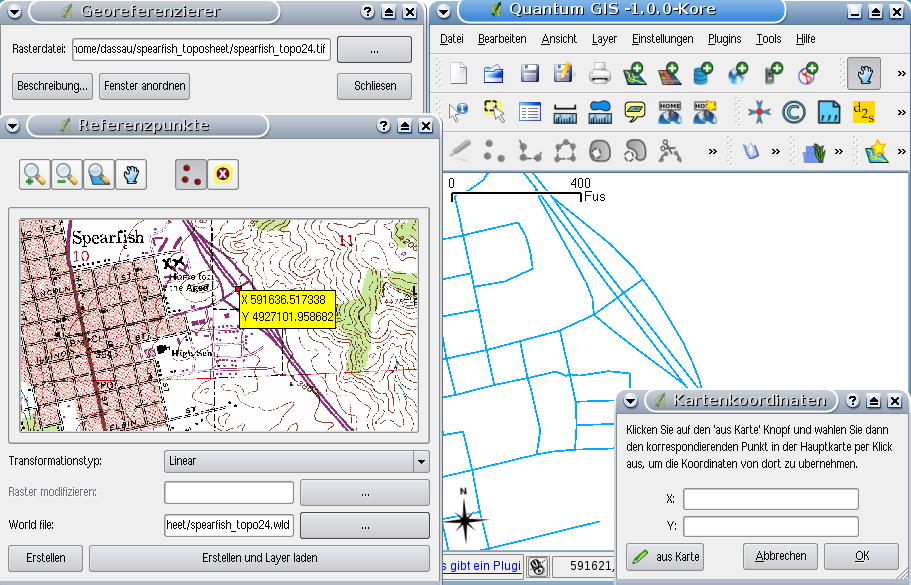
\includegraphics[clip=true, width=12cm]{georefplugin}
\end{center}
\end{figure}

\minisec{Entering ground control points (GCPs)}\label{georeferencer_entering}

\begin{enumerate}
\item To start georeferencing an unreferenced raster, we must load it using the \browsebutton browse button. The raster will show up in the main working area of the dialog. Once the raster is loaded, we can start to enter reference points.

\item Using the \toolbtntwo{mActionCapturePoint}{Add Point} button, add points to the main working area and enter their coordinates (See Figure \ref{fig:choose_points}). For this procedure you have two options:

\begin{enumerate}
\item Click on a point in the raster map and enter the X and Y coordinates manually
\item Click on a point in the raster map and choose the button \toolbtntwo{pencil}{from map canvas} to add the X and Y coordinates with the help of a georeferenced map already loaded in QGIS.
\end{enumerate}
\item Continue entering points. You should have at least 4 points, and the more coordinates you can provide, the better the result will be. There are additional tools on the plugin dialog to zoom and pan the working area in order to locate a relevant set of GCP points.
\end{enumerate}

\begin{figure}[ht]
\begin{center}
  \caption{Add points to the raster image \nixcaption}\label{fig:choose_points}\smallskip
  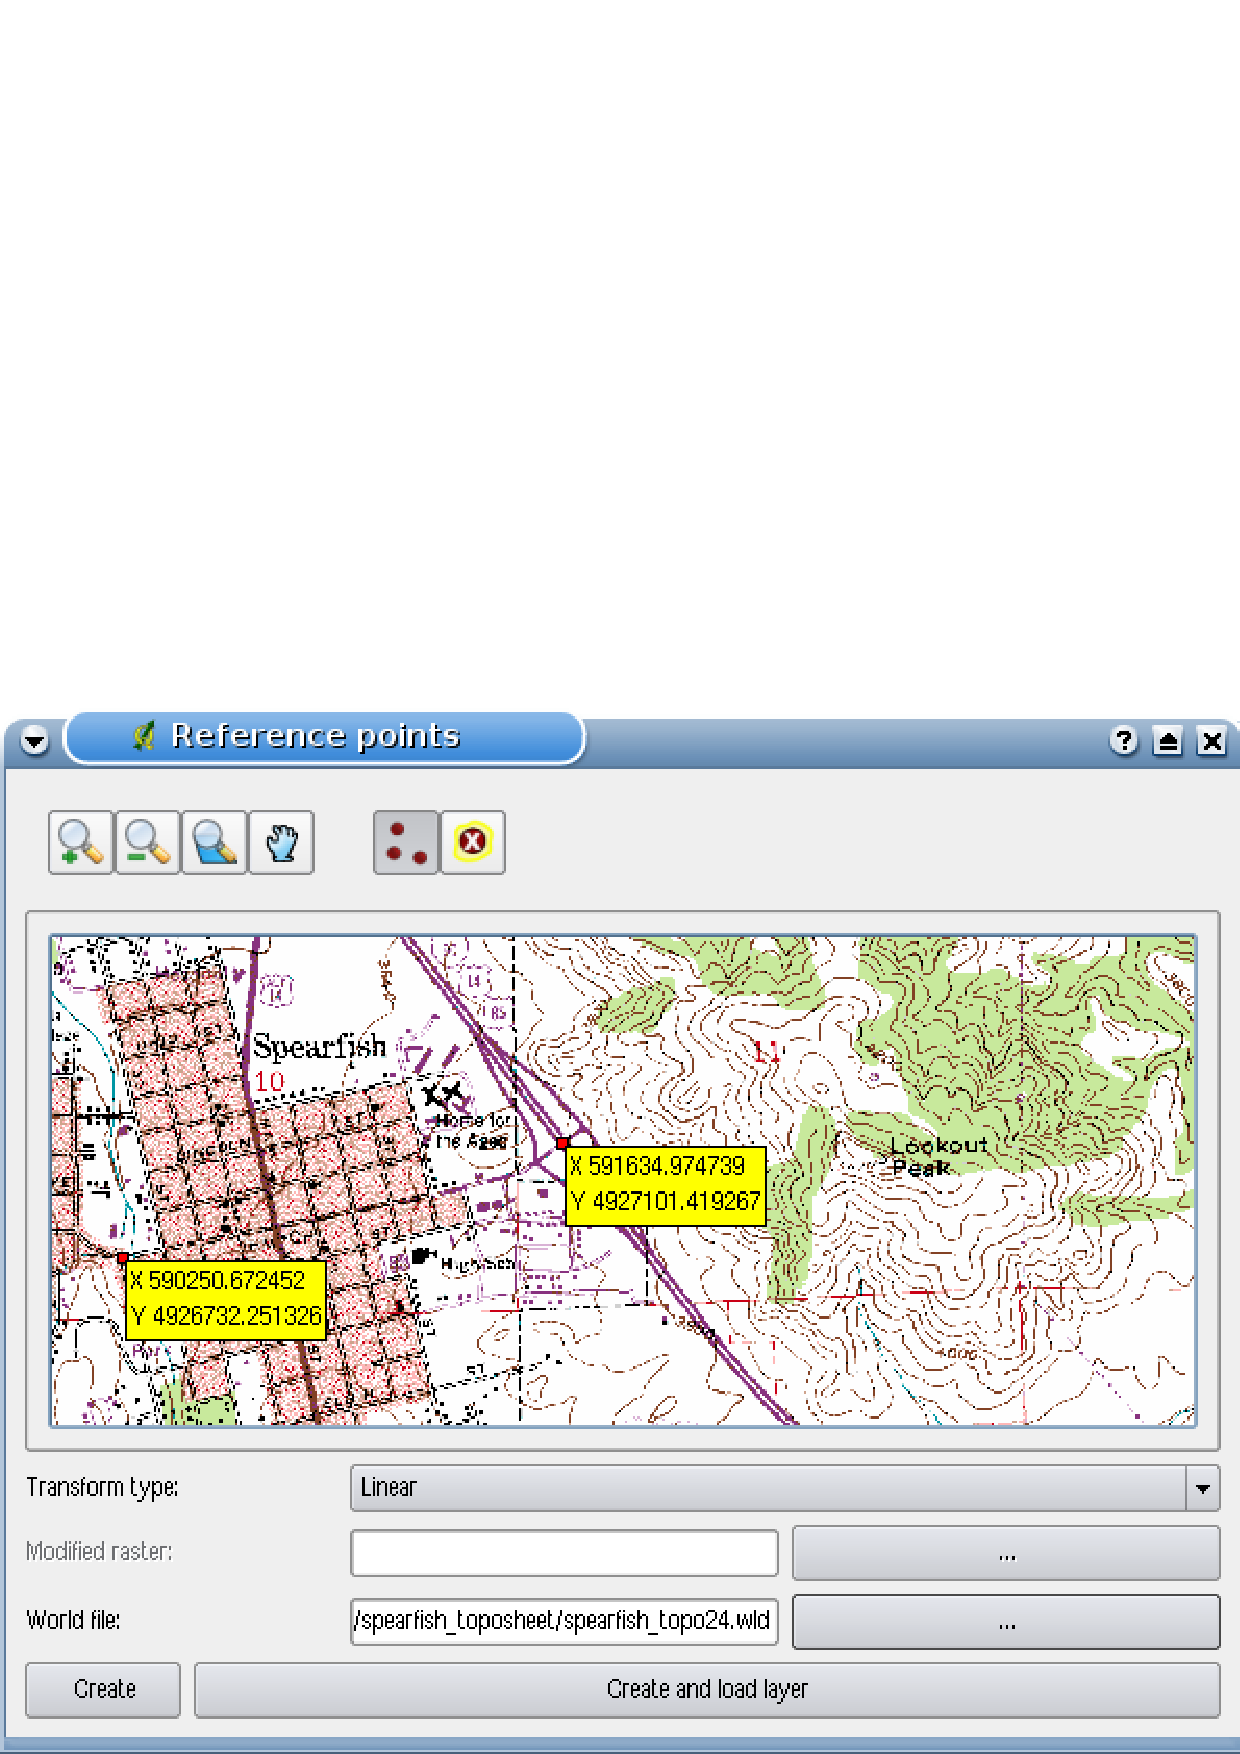
\includegraphics[clip=true,width=9cm]{choose_points}
\end{center}
\end{figure}

The points that are added to the map will be stored in a separate text file ([filename].points) which is stored together with the raster image. This allows us to reopen the Georeferencer plugin at a later date and add new points or delete existing ones to optimize the result. The points file contains values of the form: mapX, mapY, pixelX, pixelY. You can also \button{Load GCPs} and \button{Save GCPs} to different directories if you like.

\minisec{Choosing the transformation}\label{georeferencer_transformation}

After you have added your GCPs to the raster image, you need to select the transformation type for the georeferencing process. Depending on how many ground control point you have captured, you may want to use different transformation algorithms. Choice of transformation algorithm is also dependent on the type and quality of input data and the amount of geometric distortion that you are willing to introduce to final result.

Currently, several algorithms are available:

\begin{enumerate}
\item Linear
\item Helmert
\item Polynomial 1
\item Polynomial 2
\item Polynomial 3
\item Thin plate spline (TPS)
\end{enumerate}

\begin{itemize}
\item The Linear algorithm is used to create a world-file, and is different from the other algorithms, as it does not actually transform the raster. This algorithm likely won't be sufficient if you are dealing with scanned material.
\item The Helmert transformation performs simple scaling and rotation transformations. 
\item The Polynomial algorithms are among the most widely used algorithms for georeferencing, and each one differs by the degree of distortion introduced to match source and destination ground control points. The most widely used polynomial algorithm is the second order polynomial transformation, which allows some curvature. First order polynomial transformation (affine) preserves colliniarity and allows scaling, translation and rotation only.
\item The Thin plate spline (TPS) algorithm is a more modern georeferencing method, which is able to introduce local deformations in the data. This algorithm is useful when very low quality originals are being georeferenced.
\end{itemize}

\minisec{Running the transformation}\label{georeferencer_running}

\begin{enumerate}
\item When the GCPs have been collected, and the transformation has been chosen, press either \button{Create} to create a new raster or \button{Create and load layer} to automatically add the new raster to the layer list.
\item A warning message will appear that will inform you that a new raster (in GeoTIFF format) will be created.
\item After hitting OK, you will also be asked to choose a resampling method. There are three methods available:

\begin{enumerate}
\item Nearest neighbour
\item Linear
\item Cubic
\end{enumerate}
\end{enumerate}

\begin{Tip}\caption{\textsc{Choosing the resampling method}}
\qgistip{The type of resampling you choose will likely depending on your input data and the ultimate objective of the exercise. If you don't want to change statistics of the image, you might want to choose Nearest neighbour, whereas a Cubic resampling will likely provide a more smoothed result.}
\end{Tip}


